\documentclass[12pt]{article}
\usepackage[hidelinks]{hyperref}
\usepackage{graphicx, amsmath, listings, amssymb, commath}
\usepackage[utf8]{inputenc}
\usepackage[slovene]{babel}
\usepackage{amsmath}
\usepackage{enumitem}
\usepackage[utf8]{inputenc}
\usepackage{graphicx}
\usepackage{listingsutf8}
\usepackage{float}
\setlist[enumerate]{font=\large\bfseries}
\setlist[itemize]{font=\normalsize\bfseries}
\lstdefinestyle{mystyle}{
	showtabs=false, 
	tabsize=2
}

\lstdefinestyle{mystyle}{
	showtabs=false, 
	tabsize=2
}
\lstset{style=mystyle}
\usepackage[utf8]{inputenc}

\title{\small{2. projekt pri predmetu MATEMATIČNO MODELIRANJE} \\ \hfill \\ \hfill \\ \huge{\textbf{Presek dveh implicitno danih ploskev}}}
\author{Aljaž Verlič, Lina Lumborovska, Blažka Blatnik, Luka Tavčer \\
	Mentor: Damir Franetič}
\date{5. junij, 2017}
\begin{document}

\maketitle

\textbf{\large{Vsebina}} 
\begin{enumerate}
	\item Predstavitev problema
	\item Opis modela in uporabljenih metod
	\item Potrebni pogoj in Jacobijeva matrika
	\item Adaptivni korak
	\item Implementacija, testiranje in primeri
	\item Analiza za povpre\v{c}no \v{s}tevilo korakov Newtonove metode
	\item Koda
	\item Delitev dela v skupini
	\item Reference
\end{enumerate} 
\newpage

\section{Predstavitev problema}
	V $\mathbb{R}^3$ imamo podani dve poljubni implicitno dani ploskvi, opisani z enačbama $f_{1}(x)$ = $C_{1}$ in $f_{2}(x)$ = $C_{2}$. Presek teh dveh ploskev je množica rešitev nelinearnega sistema enačb:
	\begin{center}
		$f_{1}(x)$ = $C_{1}$,\\$f_{2}(x)$ = $C_{2}$.
	\end{center}
	Naša naloga je poiskati krivuljo $K$ (oz. bolj natan\v{c}no to\v{c}ke na njej), ki predstavlja presek teh dveh ploskev. \\

\section{Opis modela in uporabljenih metod}
    Sistem lahko gledamo tudi, kot enačbe nivojnic funkcij  $f_{1}$ in $f_{2}$, krivulja K pa je presek teh nivojnic. Gradienta funkcij sta tako v vsaki točki krivulje preseka, pravokotna nanjo. To opišemo:
    \begin{center}
        	$F(x) = \dfrac{(grad f_{1}(x))\times(grad f_{2}(x))}{\|grad f_{1}(x))\times(grad f_{2}(x))\|}$
    \end{center}
   in označimo $x = x(t)$ naravno parametrizacijo krivulje K. Ta x je rešitev avtonomnega sistema diferencialnih enačb:
   \begin{center}
		$\dot{x} = F(x)$
	\end{center}
	
\subsection{Re\v{s}evanje sistema diferencialnih ena\v{c}b}
    Za re\v{s}evanje sistema diferencialnih ena\v{c}b, lahko uporabimo katero izmed dveh znanih metod za numeri\v{c}no re\v{s}evanje diferencialnih ena\v{c}b.
\subsubsection{Eulerjeva metoda}
    Eulerjeva metoda je numeri\v{c}na metoda za re\v{s}evanje diferencialnih ena\v{c}b, z podanim za\v{c}etnim pribli\v{z}kom. Prednost metode je, da je preprosta in najbol logi\v{c}na. Na vsakem koraku naslednjo to\v{c}ko $(x_{i+1},y_{i+1})$ dobimo tako, da se za h (korak) premaknemo vzdol\v{z} tangente na re\v{s}itev $(x_{i},y_{i})$. Geometrijsko si lahko delovanje metode predstavimo s spodnjo sliko.
    
    \begin{figure}[H]
	    \centering
    	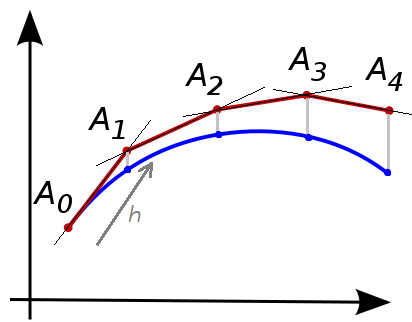
\includegraphics[width=0.5\textwidth]{Euler_method_geom}
    	\caption{Geometrijski prikaz delovanja Eulerjeve     metode $r$.}
    	\label{slika:Euler_method_geom}
	\end{figure}

	Slabost opisanega postopka je gotovo napaka, ki se skozi iteracije izvajanja metode pove\v{c}uje (napaka na vsakem koraku metode je reda $O(h^2)$, komulativna napaka pa z vsako iteracijo nara\v{s}\v{c}a). Tako je napaka ve\v{c}ja, tem ve\v{c}ji je korak. V iskanju re\v{s}itve na\v{s}ega problema to predstavlja te\v{z}avo, zato je potrebno sproti nara\v{c}unane pribli\v{z}ke vedno popraviti tako, da spet le\v{z}ijo na krivulji preseka. 
	Iz preprostega primera iskanja presečišča valja in sfere lahko opazimo delovanje Eulerjeve metode in problem komulativne napake: (Valja na sliki zaradi ve\v{c}je preglednosti ni)
	
	\begin{figure}[H]
	    \centering
    	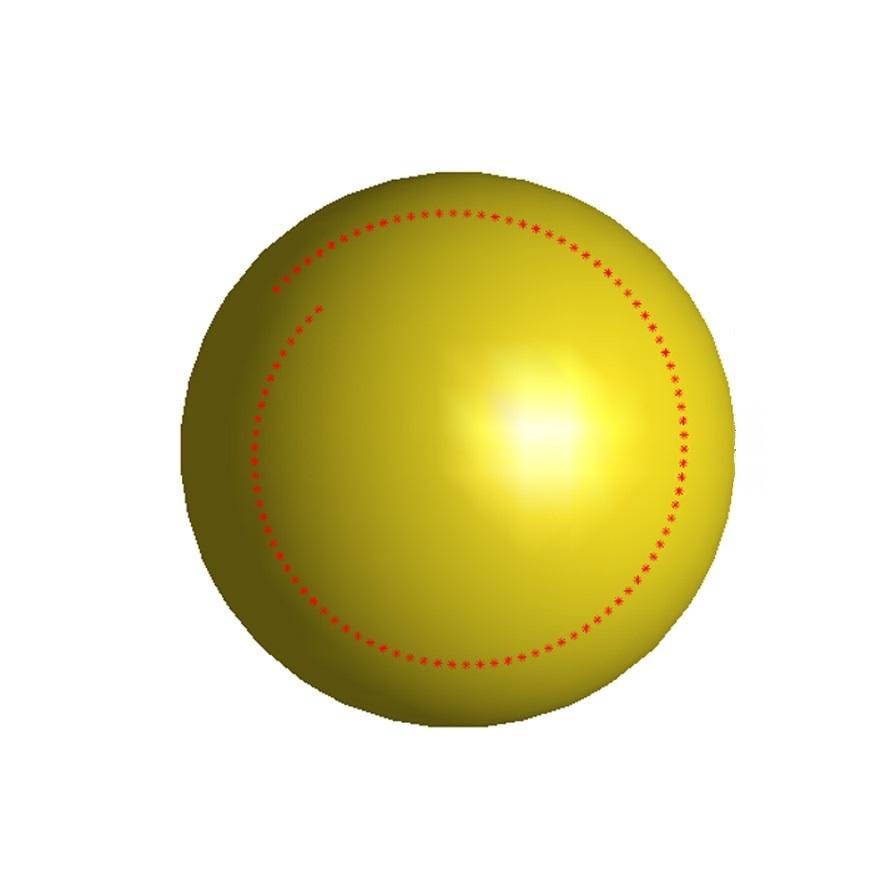
\includegraphics[scale=0.30]{eul1}
    	\caption{Eulerjeva metoda pri manjsem koraku}
    	\label{slika:eul1}
	\end{figure}
	\begin{figure}[H]
	    \centering
    	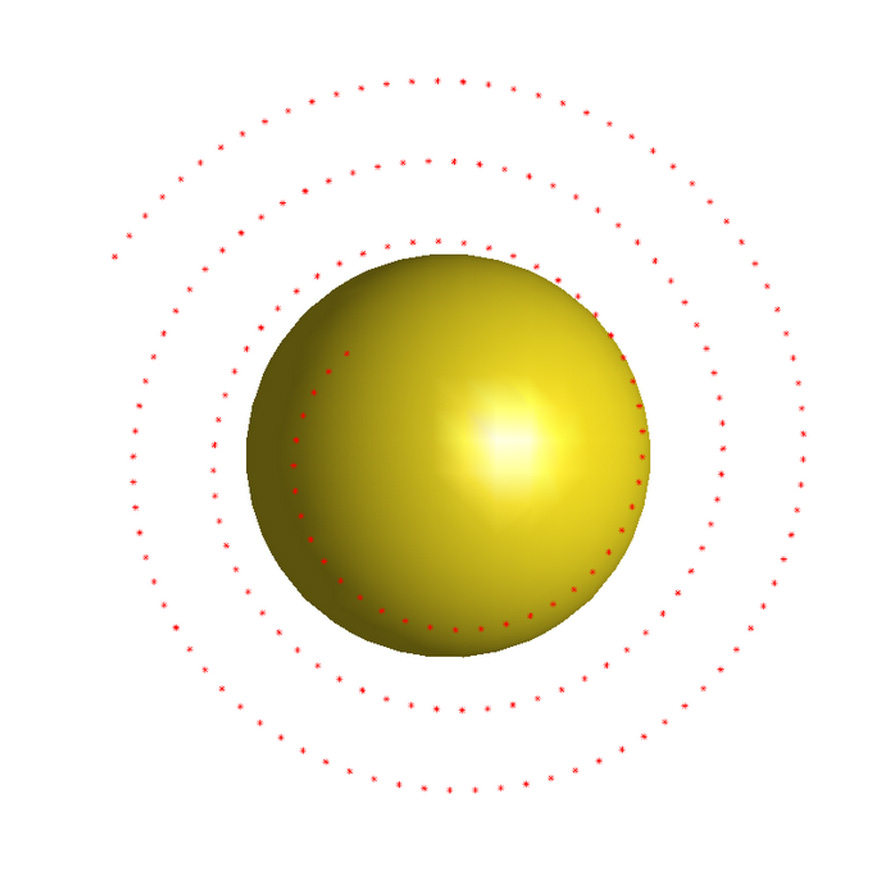
\includegraphics[scale=0.30]{eul2}
    	\caption{Eulerjeva metoda pri večjem koraku}
    	\label{slika:eul2}
	\end{figure}

	
\subsubsection{Metoda Runge-Kutta 4}
    Precej bol natan\v{c}na, a manj intuitivna, metoda za re\v{s}evanje diferencialnih ena\v{c}b je metoda Runge-Kutta 4. Tudi tu potrebujemo nek za\v{c}etni pribli\v{z}ek, metoda pa potem z ve\v{c}jo natan\v{c}nostjo ra\v{c}una nadaljne premike. Napaka na vsakem koraku je enaka Eulerjevi metodi, vendar je komulativna napaka konstantna in se z iteracijami ne povečuje.

\subsubsection{Newtnova metoda za popravljanje pribli\v{z}ka}
    Kot je mo\v{c} opaziti, je pri uporabi Eulerjeve metode potrebno sprotno popravljanje pribli\v{z}kov, druga\v{c}e se napaka se\v{s}teva do te mere, da ne dobimo \v{z}eljene re\v{s}itve.\\
    Dobljeni pribli\v{z}ek y, \v{z}elimo popraviti na nek x, ki bo le\v{z}al na preseku. \v{C}e zapi\v{s}emo $F(y) \cdot x = F(y)\cdot y $, nam to predstavlja ena\v{c}bo ravnine, ki je zelo bliz normalni ravnini na krivuljo K. Z Newtonovo metodo z za\v{c}etnim pribli\v{z}kom y re\v{s}imo sistem ena\v{c}b:
    \begin{center}
    	$f_{1}(x)$ = $C_{1}$\\$f_{2}(x)$ = $C_{2}$\\ $F(y) \cdot x = F(y)\cdot y $
    \end{center}
    Re\v{s}itev sistema je to\v{c}ka, ki le\v{z}i na prese\v{c}i\v{s}\v{c}u obeh ploskev. V primeru uporabe RK4 je Newtnova metoda potrebna bolj za postavitev zacetnega pribli\v{z}ka na prese\v{c}i\v{sc}e, saj je metoda RK4 sama po sebi precej natan\v{c}na. U\v{c}inkovitost metode je razvidna iz primerov:
    
    \begin{figure}[H]
        \centering
        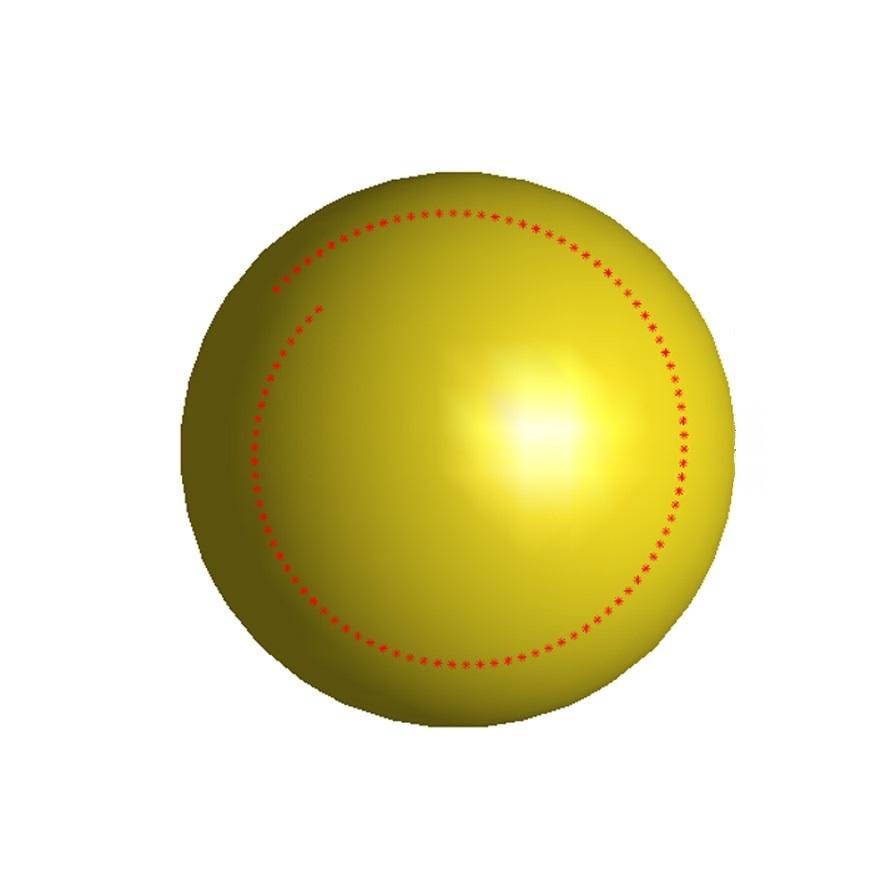
\includegraphics[scale=0.3]{eul1}
	    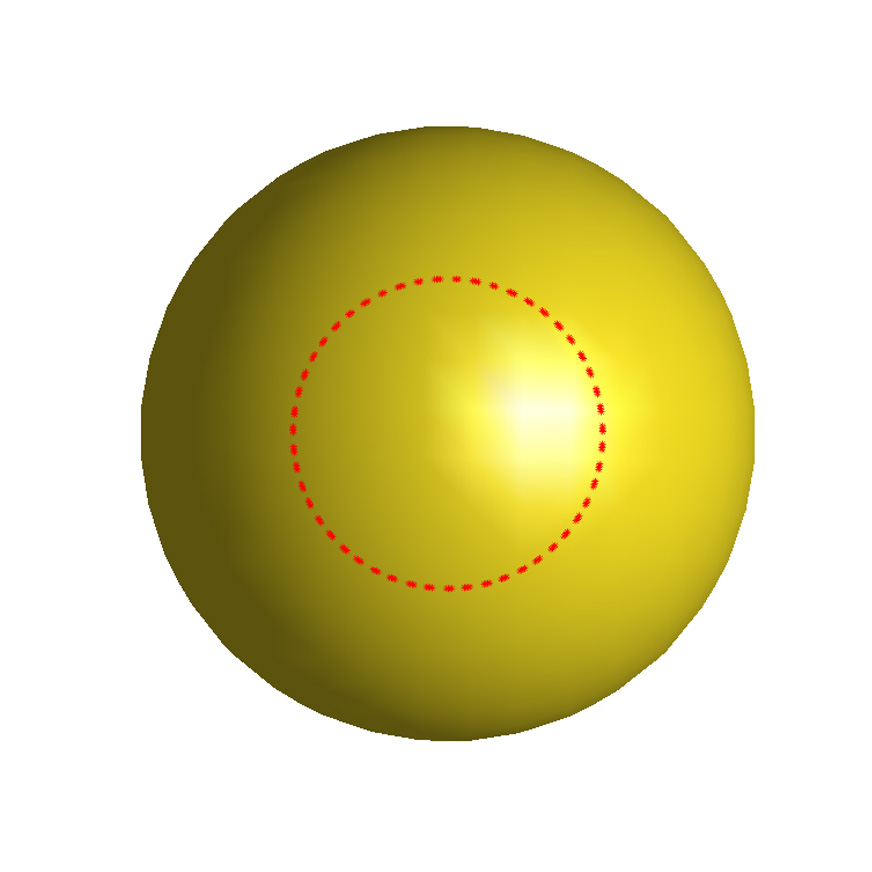
\includegraphics[scale=0.3]{eul3_newt}
	    \caption{Osnovna Eulerjeva metoda (levo) in popravljena Eulerjeva metoda (desno).}
    	\label{slika:eul1,eul3_newt}
	\end{figure}
    \begin{figure}[H]
        \centering
        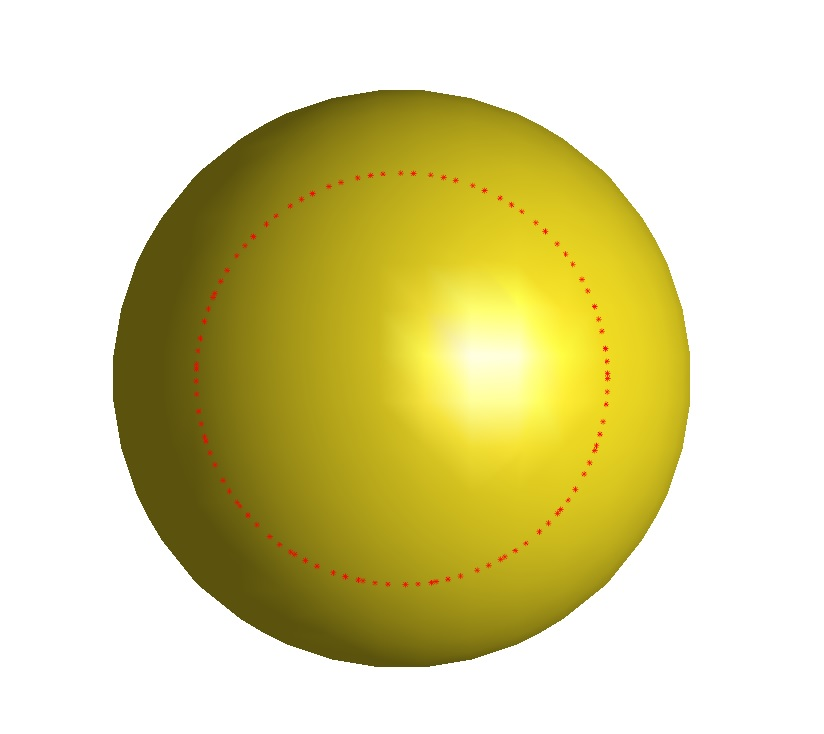
\includegraphics[scale=0.30]{rk4}
    	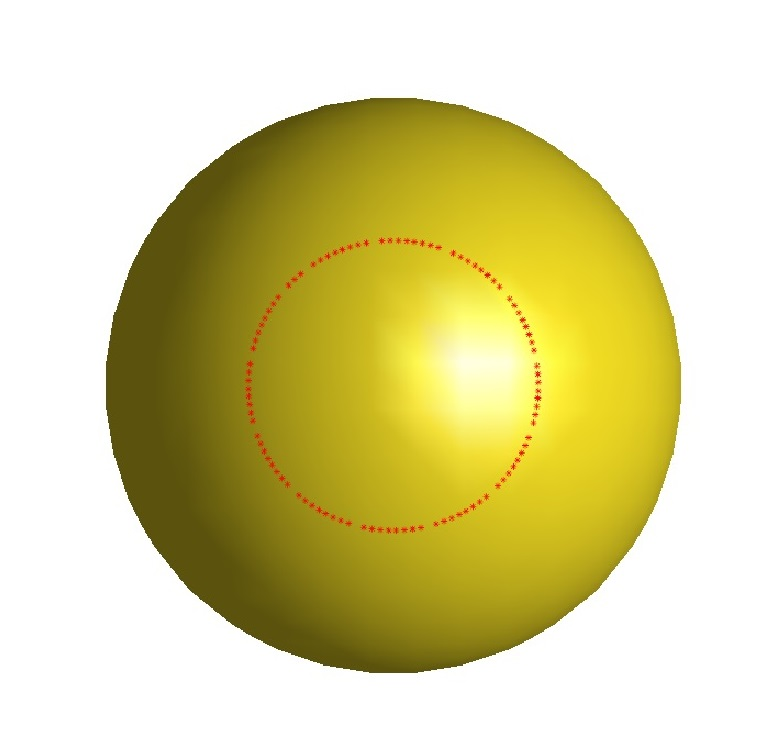
\includegraphics[scale=0.30]{rk4_newt}
	    \caption{Osnovna metoda RK4 (levo) in popravljena metoda RK4 (desno).}
    	\label{slika:rk4,rk4_newt}
	\end{figure}

\newpage	
\section{Potrebni pogoj in Jacobijeva matrika}
	Potreben pogoj za delovanje metod je, da sta funkciji $f_{1}$ in $f_{2}$ parcialno odvedljivi in da ima Jacobijeva matrika parcialnih odvodov poln rang 2. Za uspešno delovanje Newtonove metode moramo poiskati Jacobijevo matriko leve strani sistema nelinearnih enačb:

	\begin{center}
		JG = $\begin{bmatrix}
		grad(f_{1}) \\
		grad(f_{2}) \\
		\hspace{1mm}grad(\vec{v} \cdot \vec{x}) \\
		\end{bmatrix}$
		oziroma
		JG = $\begin{bmatrix}
		grad(f_{1}) \\
		grad(f_{2}) \\
		\hspace{1mm}grad(\vec{v}\hspace{0.5mm}^\intercal) \\
		\end{bmatrix}$
	\end{center}
	Newtnova metoda rešuje sistem:
	\begin{center}
	    $\vec{F}(\vec{x}) = \vec{0}$,
	\end{center}
	zato je potrebno poiskati tudi matriko $\vec{F}(\vec{x})$, ki je enaka:
		\begin{center}
		$\vec{F}(\vec{x})$ = $\begin{bmatrix}
		f_{1}(\vec{v}) - C_{1} \\
		f_{2}(\vec{v}) - C_{2} \\
		\hspace{1mm}\vec{v} \cdot \vec{x} - \vec{v} \cdot \vec{y}) \\
		\end{bmatrix}$
	\end{center}

\section{Adaptivni korak}
    Adaptivni korak omogoča bolj natančno rešitev problema, saj dinamično prilagaja dolžino koraka. Tako lahko na bolj preprostih predelih preseka uporabljamo večji h (korak) in je metoda hitrejša, na bolj kompleksnih delih preseka, kjer je potrebna večja natančnost, pa se premikamo z manjšim korakom. Program poveča oziroma zmanjša korak glede na število korakov, ki jih izvede Newtonova metoda za eno točko. Empirično smo določili, da je velikost koraka h na intervalu $h\in[10^{-7},100]$ in da se korak povečuje oziroma zmanjšuje za faktor 2. Korak je nespremenjen, če je število korakov 2 ali 3.
	
	\begin{figure}[H]
        \centering
        \begin{minipage}{.5\textwidth}
            \centering
    	    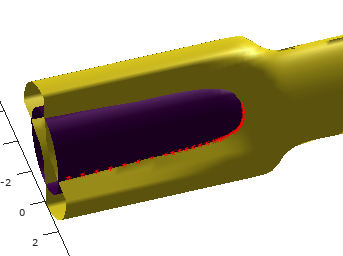
\includegraphics[scale=0.50]{slikaAda}
	        \caption{Adaptivni korak}
    	    \label{slika:slikaAda}
        \end{minipage}%
        \begin{minipage}{.5\textwidth}
            \centering
    	    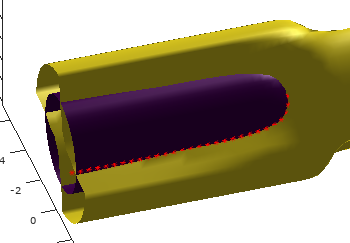
\includegraphics[scale=0.50]{slikaAda2}
	        \caption{Brez adaptivnega koraka}
    	    \label{slika:slikaAda2}
        \end{minipage}
    \end{figure}		
    
\section{Implementacija, testiranje in primeri}
	Delovanje našega programa lahko preverimo s programom, ki smo ga napisali v Octave-u. Kot vhodne parametre mu podamo obe implicitno podani funkciji $f_{1}$, $f_{2}$, $C1$, $C2$, $grad(f_{1})$, $grad(f_{2})$. Določimo tudi začetni približek $x_{0}$, začetno dolžino koraka in pa parameter, ki določa metodo delovanja (Euler/Runge-Kutta).\\
	Program poženemo na različnih primerih in štejemo povprečno dolžino koraka ter število porabljenih korakov:\\\\
		
	\begin{minipage}{\textwidth}
	\textbf{\large{Primer 1:}}
	\begin{itemize} 
		\item $f_{1}(x,y,z)$ = $x^2 + y^2 + z^2$ = 4
		\item $f_{2}(x,y,z)$ = $3x + 2y + z$ = 1	
	\end{itemize}
	\begin{figure}[H]
	    \centering
    	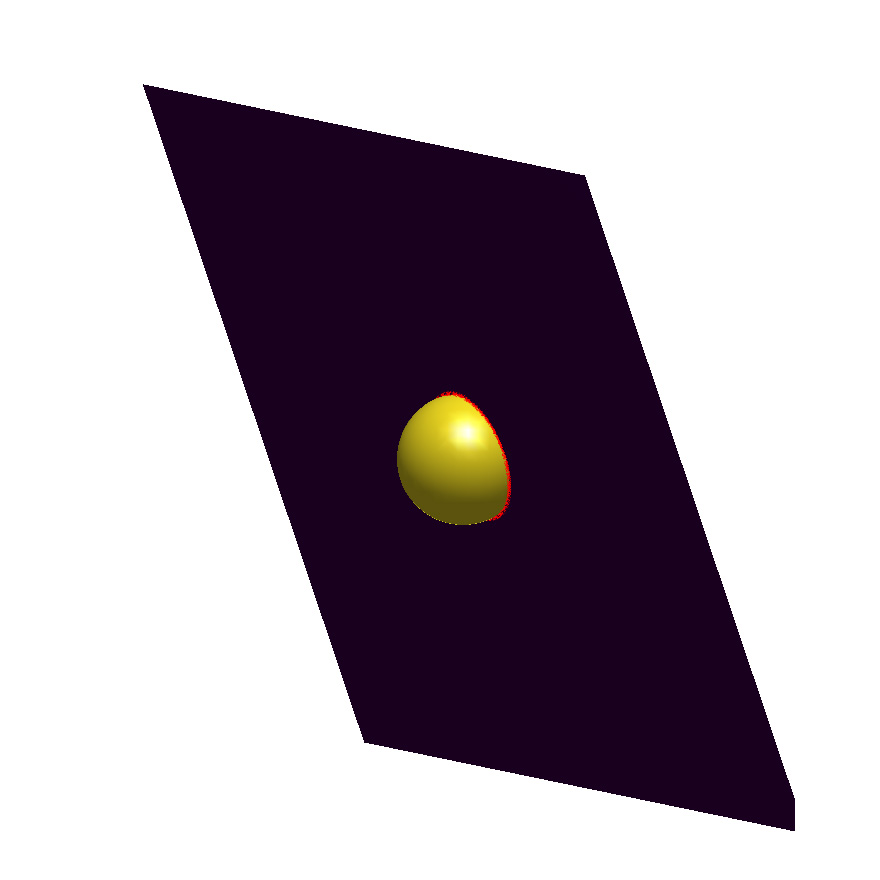
\includegraphics[scale=0.3]{primer1_1}
    	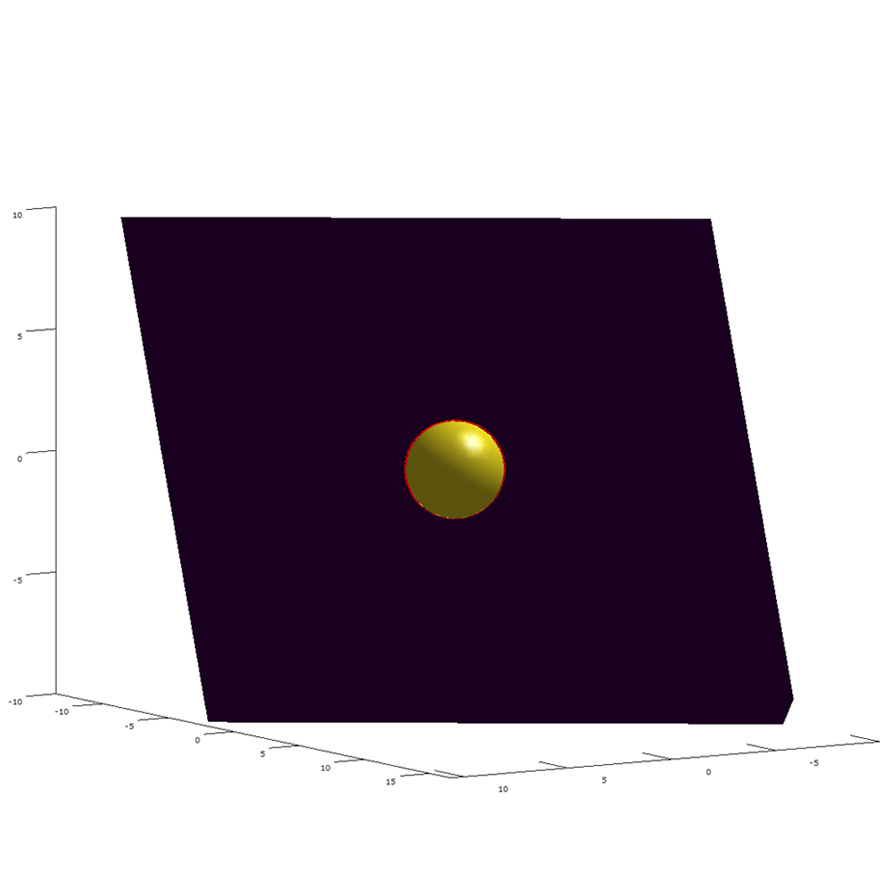
\includegraphics[scale=0.3]{primer1_2}
    \end{figure}
    \end{minipage}
    
	\begin{minipage}{\textwidth}
	\textbf{\large{Primer 2:}}
	\begin{itemize}  
		\item $f_{1}(x,y,z)$ = $x^2 + y^2 + z^2$ = 4
		\item $f_{2}(x,y,z)$ = $x^2 + y^2$ = 1
	\end{itemize}
	\begin{figure}[H]
	    \centering
	    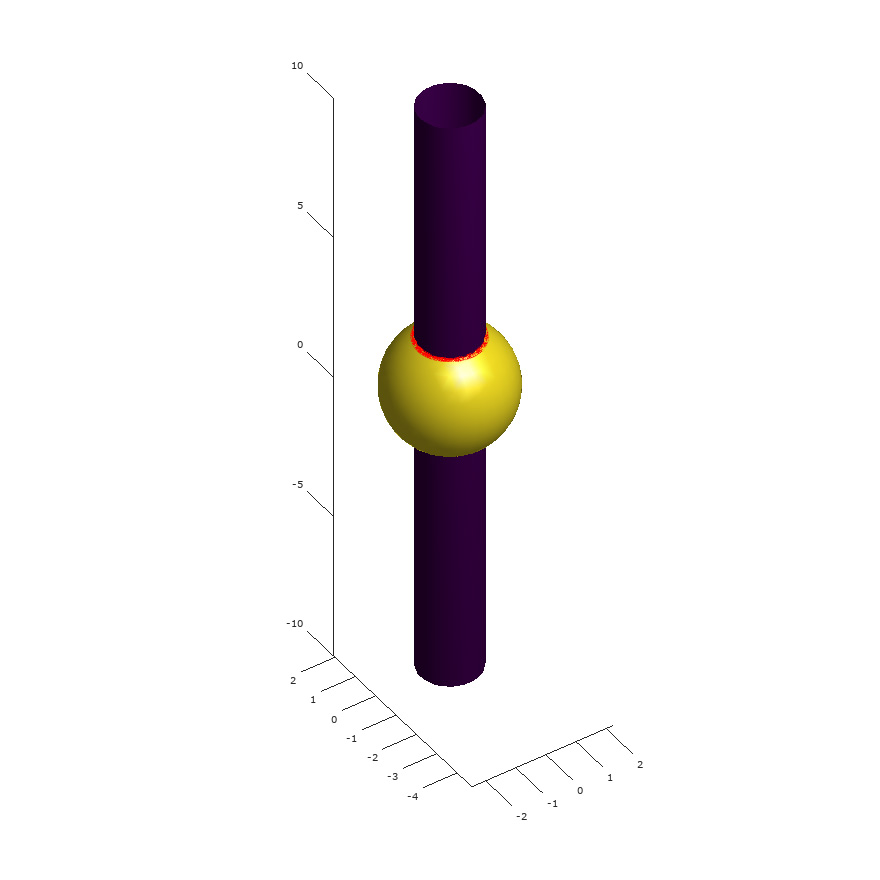
\includegraphics[scale=0.3]{primer2_1}
    	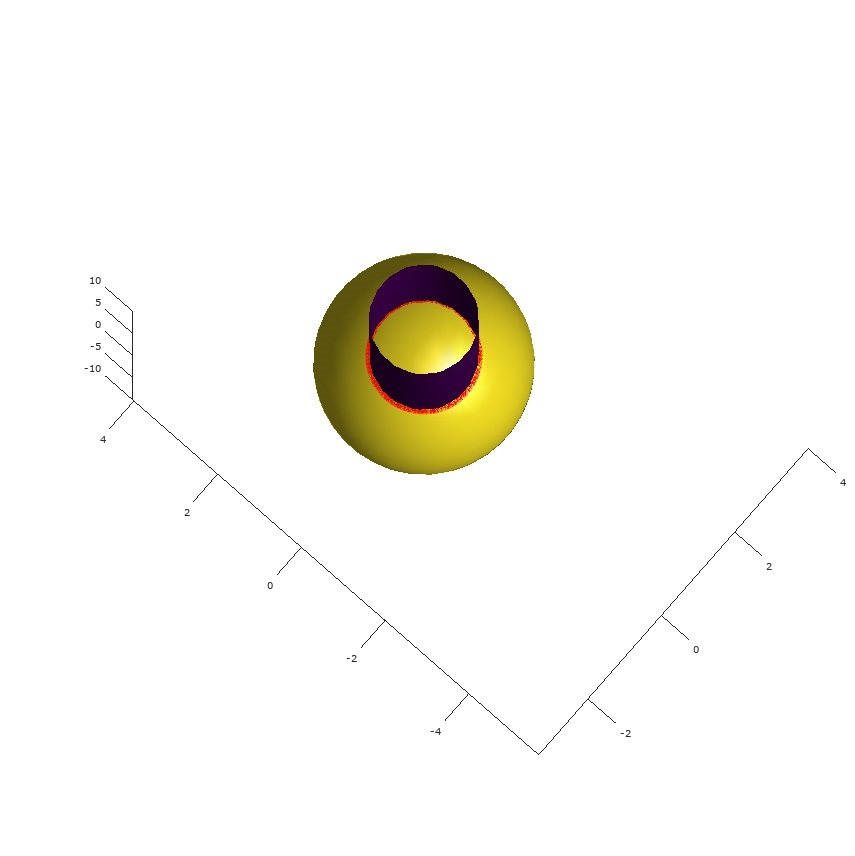
\includegraphics[scale=0.3]{primer2_2}
	\end{figure}
	\end{minipage}
	
		\begin{minipage}{\textwidth}
	\textbf{\large{Primer 3:}}
	\begin{itemize}  
		\item $f_{1}(x,y,z)$ = $x^2 + y^2 + z^2$ = 4
		\item $f_{2}(x,y,z)$ = $y^4 + log(x^2 + 1)z^2 - 4$ = 1
	\end{itemize}
	\begin{figure}[H]
	    \centering
	    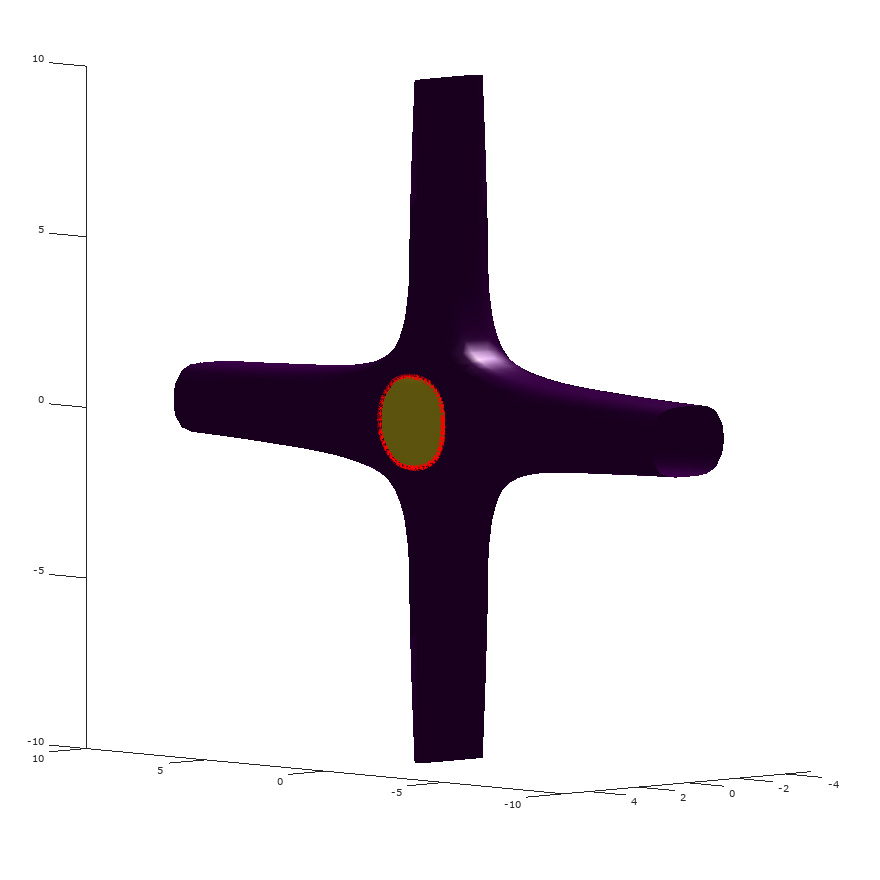
\includegraphics[scale=0.3]{primer3_1}
    	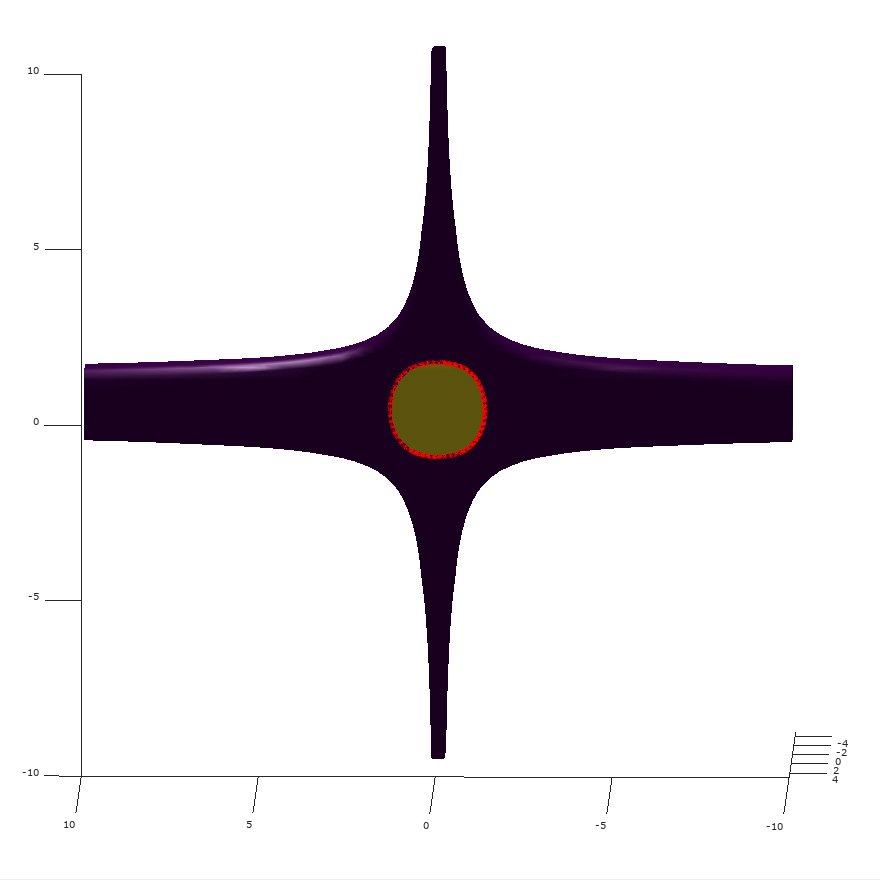
\includegraphics[scale=0.3]{primer3_2}
	\end{figure}
	\end{minipage}
	
	\begin{minipage}{\textwidth}
	\textbf{\large{Primer 4:}}
	\begin{itemize}  
		\item $f_{1}(x,y,z)$ = $x^2 + cos(y)z^2 - 12$ = 4
		\item $f_{2}(x,y,z)$ = $y^4 + log(x^2 + 1)z^2 - 4$ = 1
	\end{itemize}
	\begin{figure}[H]
	    \centering
    	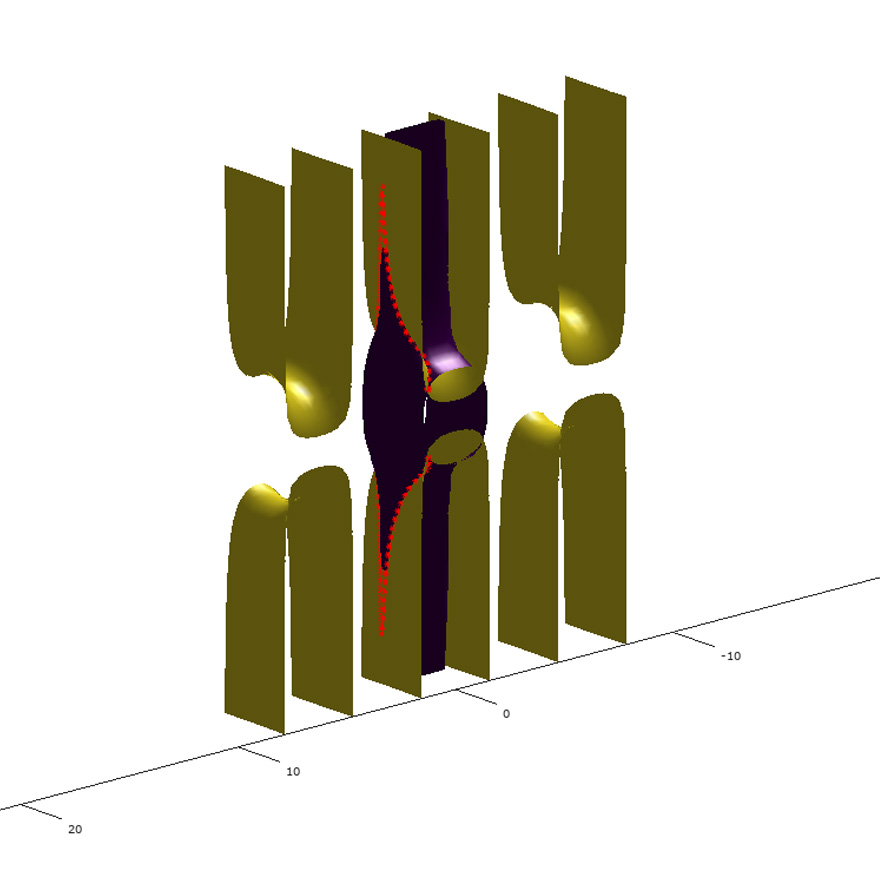
\includegraphics[scale=0.3]{primer4_1}
    	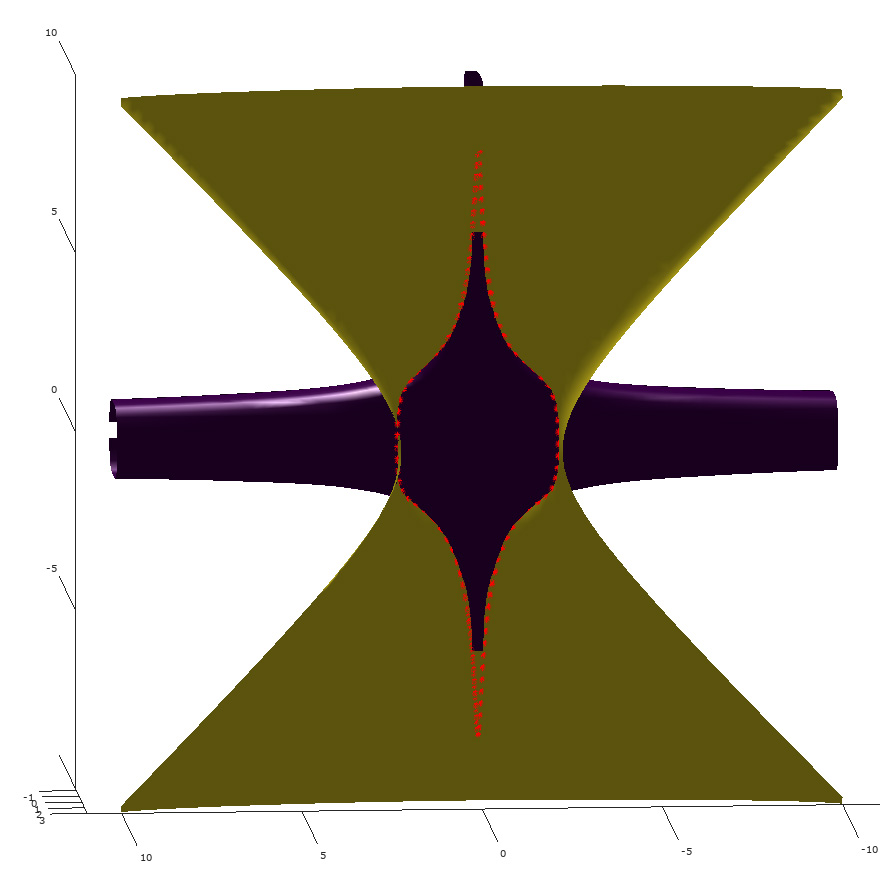
\includegraphics[scale=0.3]{primer4_2}
    	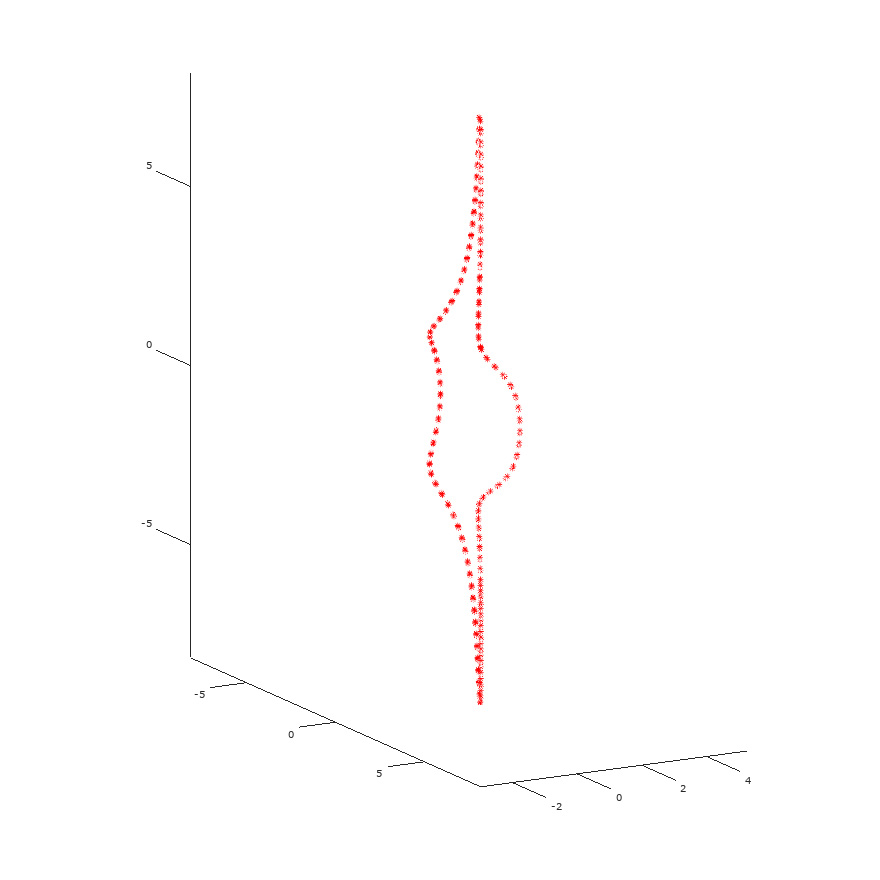
\includegraphics[scale=0.3]{primer4_4}
    	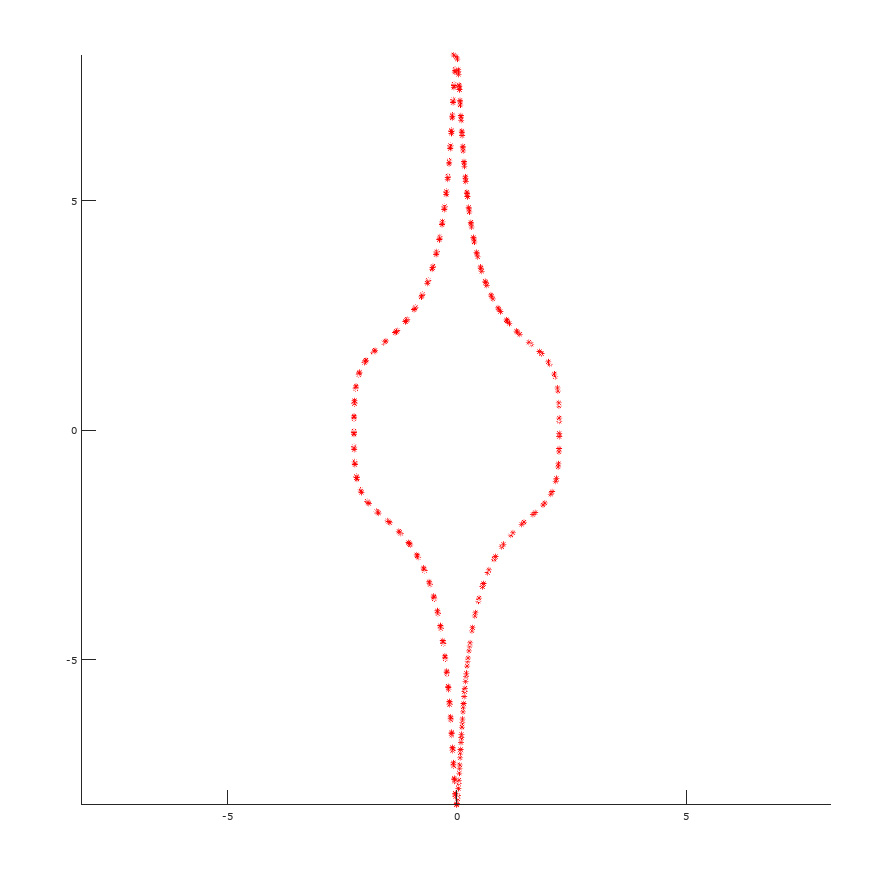
\includegraphics[scale=0.3]{primer4_3}
	\end{figure}
	\end{minipage}
	
	\begin{minipage}{\textwidth}
	\textbf{\large{Primer 5:}}
	\begin{itemize}  
		\item $f_{1}(x,y,z)$ = $e^{(-x^{2}+1)}+y^{2}+z^{2}$ = 3
		\item $f_{2}(x,y,z)$ = $e^{(xyz)}+y^{2}+z^{2}$ = 10
	\end{itemize}
	\begin{figure}[H]
    	\centering
    	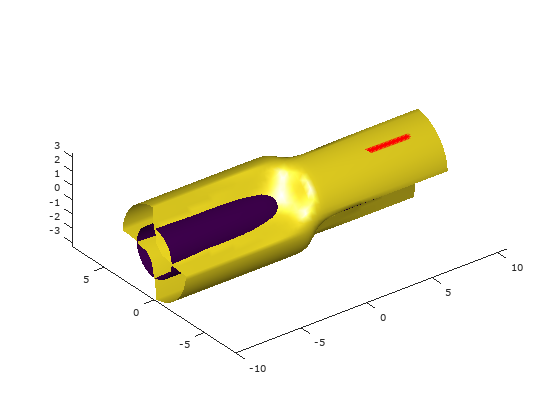
\includegraphics[scale=0.4]{primer5_1}
    	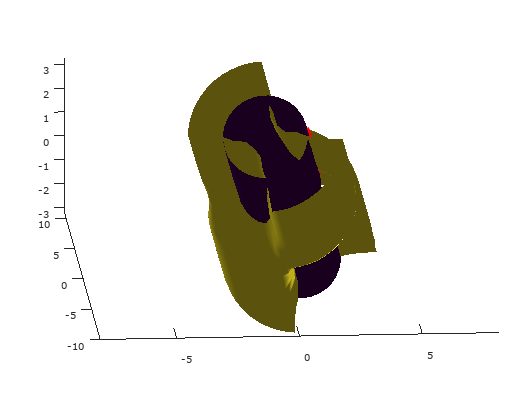
\includegraphics[scale=0.4]{primer5_2} 
    	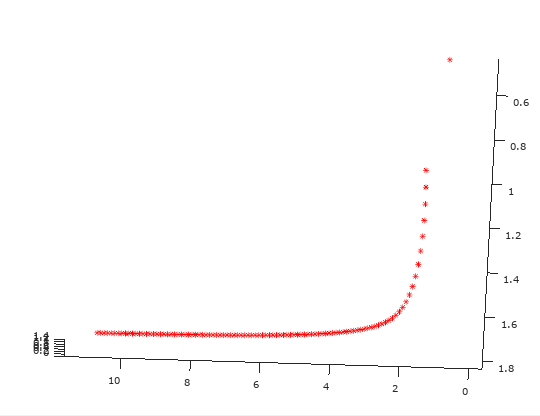
\includegraphics[scale=0.4]{primer5_3}
    	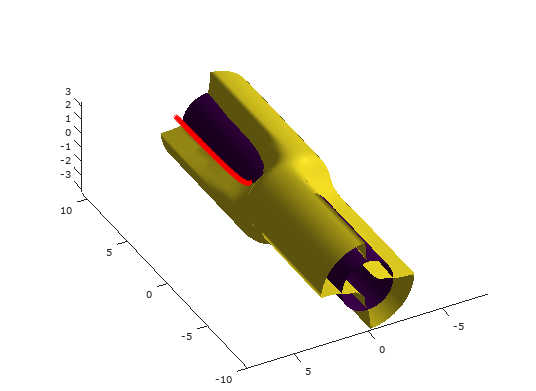
\includegraphics[scale=0.4]{primer5_4} 
	\end{figure}
	\end{minipage}
	
	\begin{minipage}{\textwidth}
	\textbf{\large{Primer 6:}}
	\begin{itemize}  
		\item $f_{1}(x,y,z)$ = $e^{(-x^{2}+1)}+y^{2}+z^{2}$ = 3
		\item $f_{2}(x,y,z)$ = $x^2 + y^2 + z^2$ = 4
	\end{itemize}
	\begin{figure}[H]
    	\centering
	    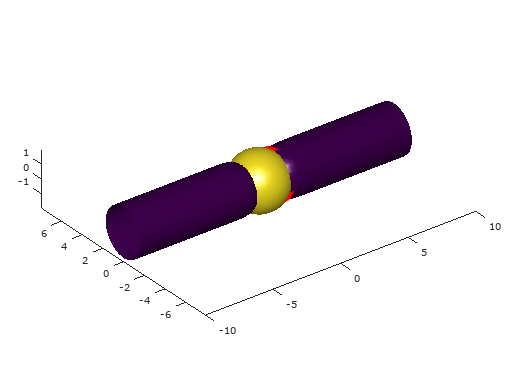
\includegraphics[scale=0.5]{primer6_1}
	    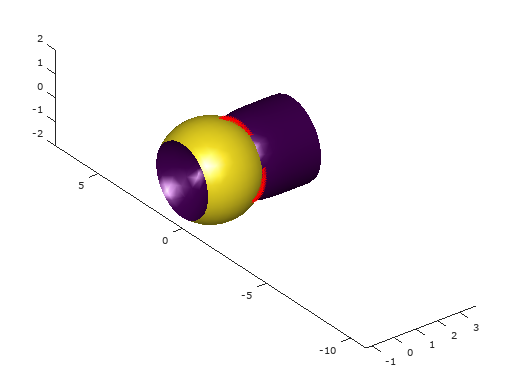
\includegraphics[scale=0.5]{primer6_2}
    	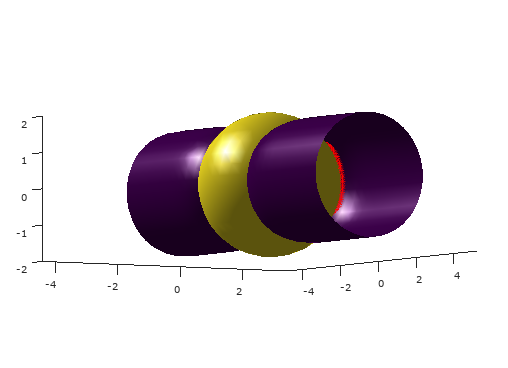
\includegraphics[scale=0.5]{primer6_3}
	    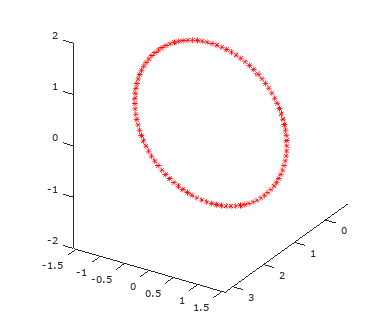
\includegraphics[scale=0.5]{primer6_4} 
	\end{figure}
	\end{minipage}
	
	\begin{minipage}{\textwidth}
	\textbf{\large{Primer 7:}}
	\begin{itemize}  
		\item $f_{1}(x,y,z)$ = $e^{(-x^{2}+1)}+y^{2}+z^{2}$ = 3
		\item $f_{2}(x,y,z)$ =  $x^2 + y^2$ = 1
	\end{itemize}
	\begin{figure}[H]
    	\centering
    	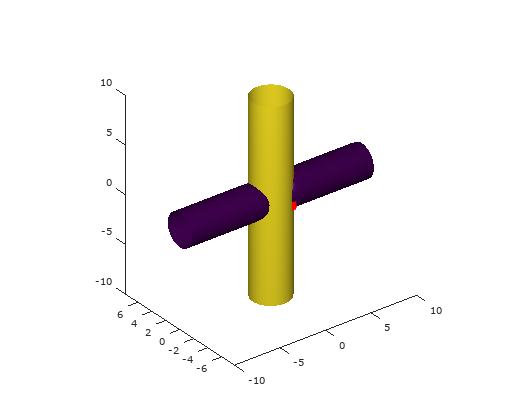
\includegraphics[scale=0.4]{primer7_1}
	    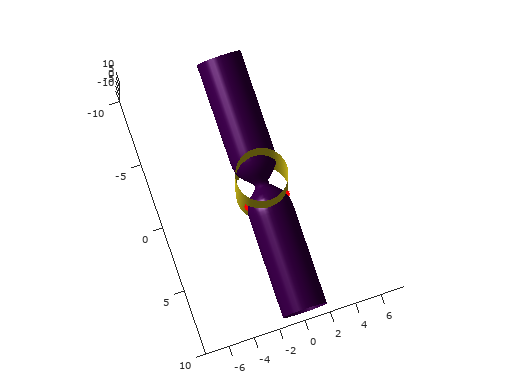
\includegraphics[scale=0.4]{primer7_2}
	    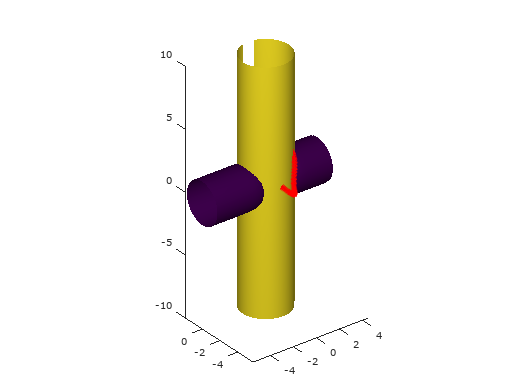
\includegraphics[scale=0.4]{primer7_3}
    	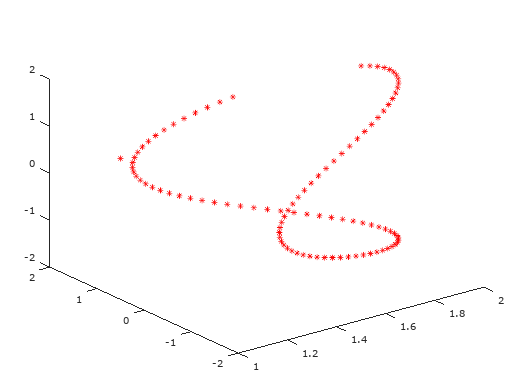
\includegraphics[scale=0.4]{primer7_4} 
    \end{figure}    
    \end{minipage}
    
	\begin{minipage}{\textwidth}
	\textbf{\large{Primer 8:}}
	\begin{itemize}  
		\item $f_{2}(x,y,z)$ = $e^{(xyz)}+y^{2}+z^{2}$ = 10
		\item $f_{2}(x,y,z)$ =  $x^2 + y^2$ = 1
	\end{itemize}
	\begin{figure}[H]
    	\centering
    	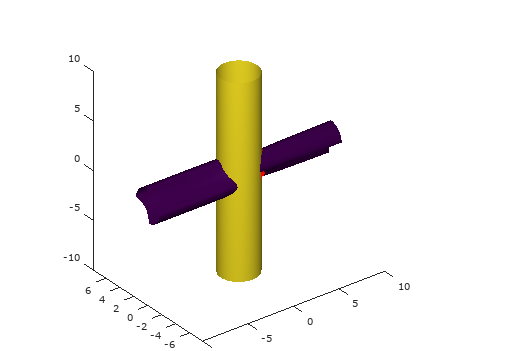
\includegraphics[scale=0.5]{primer8_1}
    	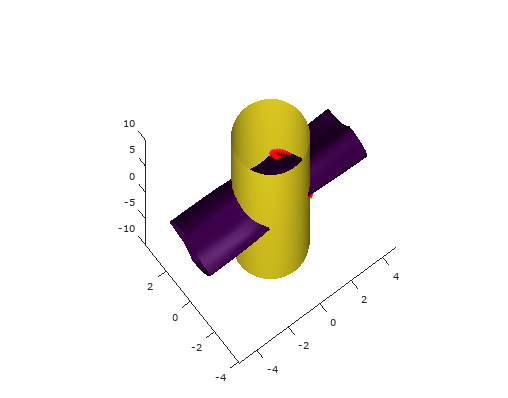
\includegraphics[scale=0.5]{primer8_2}
    	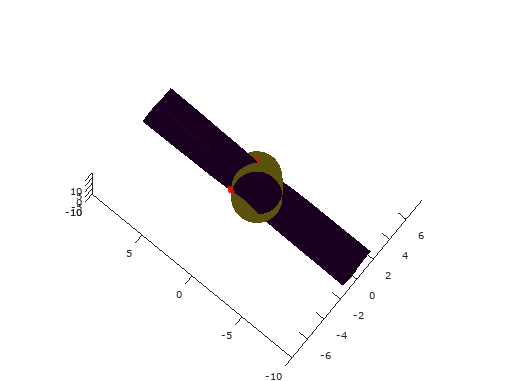
\includegraphics[scale=0.5]{primer8_3}
    	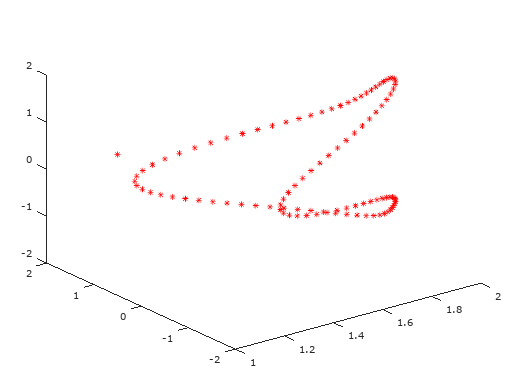
\includegraphics[scale=0.5]{primer8_4} 
    \end{figure} 
    \end{minipage}
\newpage
\section{Analiza za povpre\v{c}no \v{s}tevilo korakov Newtonove metode} 
Na koncu smo za vseh 8 primerov naredili analizo, tako da smo izmerili povpre\v{c}no \v{s}tevilo korakov Newtonove metode za RK4 in Eulerjevo matodo na dva na\v{c}ina: z adaptivnem in fiksnem korakom. Pri adaptivnem koraku smo izra\v{c}unali tudi minimalno in maksimalno \v{s}tevilo korakov.\\ \\
Primer in rezultati izvajanje enega testa: 

    \begin{figure}[H]
        \centering
        \begin{minipage}{.5\textwidth}
            \centering
            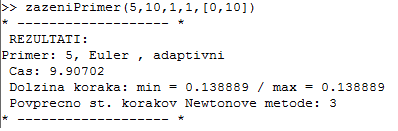
\includegraphics[scale=1]{a1}
            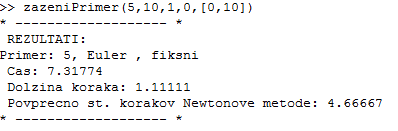
\includegraphics[scale=1]{a2}
            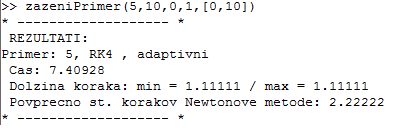
\includegraphics[scale=1]{a3}
	        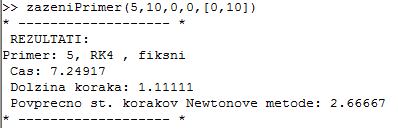
\includegraphics[scale=1]{a4}
        \end{minipage}%
    \end{figure}	
\newpage
Po izvajanje tega postopka za vse primere smo dobili naslenje rezultate: \\
\begin{tabular}{|c | c | c | c | c |} 
 \hline
 \textbf{Funkcija} &\multicolumn{2}{|l|}{\textbf{Euler}} &\multicolumn{2}{|l|}{\textbf{RK4}}\\                
  \small &adaptivno & fiksno & adaptivno & fiksno \\ 
 \hline
 \small{}$f_{1}(x,y,z)=x^{2} + y^{2}+ z^{2}=4$ & & & &\\ 
 \small{}$f_{2}(x,y,z)=x^{2} + y^{2}    =1$  & 3 & 5 & 3 & 3.222 \\
 \hline
 \small{}$f_{1}(x,y,z)=x^{2} + y^{2}+ z^{2}=4$ & & & &\\ 
 \small{}$f_{2}(x,y,z)$ = $3x + 2y + z = 1$  & 3 & 4.222 & 3 & 3.333 \\
 \hline
 \small{}$f_{1}(x,y,z)=x^{2} + y^{2}+ z^{2}=4$ & & & &\\ 
 \small{}$f_{2}(x,y,z)$ = $y^4 + log(x^2 + 1)z^2 - 4 = 1$  & 3 & 5 & 3 & 3.222 \\
 \hline
 \small{}$f_{1}(x,y,z)$ = $x^2 + cos(y)z^2 - 12 = 4$ & & & &\\ 
\small{}$f_{2}(x,y,z)$ = $y^4 + log(x^2 + 1)z^2 - 4 = 1$  & 3 & 4.111 & 2.222 & 2.556 \\
 \hline
 \small{}$f_{1}(x,y,z)$ = $e^{(-x^{2}+1)}+y^{2}+z^{2} = 3$ & & & &\\ 
 \small{}$f_{2}(x,y,z)$ = $e^{(xyz)}+y^{2}+z^{2} = 10$  & 3 & 4.667 & 2.222 & 2.667 \\
 \hline
 \small{}$f_{1}(x,y,z)$ = $e^{(-x^{2}+1)}+y^{2}+z^{2} = 3$ & & & &\\ 
 \small{}$f_{2}(x,y,z)=x^{2} + y^{2}+ z^{2}=4$  & 3 & 5 & 3 & 3.222 \\
 \hline
 \small{}$f_{1}(x,y,z)$ = $e^{(-x^{2}+1)}+y^{2}+z^{2} = 3$ & & & &\\ 
  \small{}$f_{2}(x,y,z)=x^{2} + y^{2}    =1$  & 3 & 5 & 3 & 3.333 \\
  \hline
\small{}$f_{1}(x,y,z)$ = $e^{(xyz)}+y^{2}+z^{2} = 10$ & & & &\\ 
 \small{}$f_{2}(x,y,z)=x^{2} + y^{2}    =1$  & 3 & 5 & 3 & 3.556 \\
  \hline
\end{tabular}
\newline
\newline
Pri bolj kompleksnih funkcijah kot so npr.:
\begin{itemize}
    \item $f_{1}(x,y,z)$ = $x^2 + cos(y)z^2 - 12 = 4$  in \item $f_{2}(x,y,z)$ = $y^4 + log(x^2 + 1)z^2 - 4 = 1$,
\end{itemize}
smo dobili pri adaptivnem koraku manjše povprečno število korakov, ker je metoda hitro konvergirala, vendar za to ceno zmanjšala korak in delovala počasneje (približek je bil blizu pravilne rešitve, saj je bil premik majhen). Tudi minimalno in maximalno število korakov sta bila manjša kot pri vseh ostalih. Adaptivni korak se pri teh funkcija približa spodnji meji (2), korak pa se za to ceno manjša. 
\par Pri fiksnem koraku smo prišli do podobnega zaključka kot pri adaptivnem t.j., da bolj kompleksne funkcije hitreje skonvergirajo, saj mora biti korak manjši (ni prikazano v tabeli).

\newpage
\section{Koda}
\begin{lstlisting}[language=Octave]

\end{lstlisting}
\newpage
\section{Delitev dela v skupini}
\subsection{Programerski del}
\begin{itemize}
	\item Aljaž: Adaptivni korak, test skripta
	\item Lina: Re\v{s}evanje primerov, empiri\v{c}no določanje parametrov
	\item Blažka: Ogrodje programa, zdru\v{z}itev funkcij, test skripta
	\item Luka: Re\v{s}evanje primerov, empiri\v{c}no določanje parametrov
\end{itemize}
\subsection{Poro\v{c}ilo}
\begin{itemize}
	\item Aljaž: Adaptivni korak, Jacobijeva matrika
	\item Lina: Analiza, primeri, testiranje
	\item Blažka: Predstavitev problema, opis modela in metod
	\item Luka: Opis modela in metod (primeri delovanja)
\end{itemize}
\section{Reference}
\begin{itemize}
	\item Zapiski s predavanj: Diferencialne ena\v{c}be
	\item \url{https://en.wikipedia.org/wiki/Euler_method}
\end{itemize}
\end{document}
